\documentclass{beamer}
\usepackage{mathptmx}
\usetheme{CambridgeUS}
\usecolortheme{beaver}

%Imports
\usepackage{tikz}
\usepackage{pgfplots}
\usepackage{mathtools}
\usepackage{tkz-euclide}
\usepackage{graphicx}
\usetikzlibrary{positioning}
\pgfplotsset{compat = 1.8}

\graphicspath{ {./images/} }

%Modifiers
\pgfkeys{/pgfplots/Axis Style/.style={
    width=12.5cm, height=6cm,
    axis x line=center, 
    axis y line=middle, 
    samples=100,
    ymin=-1.5, ymax=1.5,
    xmin=-4.0, xmax=4.0,
    domain=-pi:pi,
    legend style={at={(0.00,0.00)},anchor=west}
}}
\tikzset{arrowMe/.style={postaction=decorate,decoration={markings, mark=at position .5 with {\arrow[thick]{#1}}}}}

\title{Tutorat CBI}
\author{Hugo Demaret}
\date{Septembre 2022}

\begin{document}
    \begin{titlepage}
        \begin{center}
            \texttt{hugo.demaret@defi-lovelace.fr}\\
            Université Paris Cité - UFR Mathématiques Informatique
            
            \vspace*{0.5cm}
            
            
\includegraphics[scale=0.02]{./src/cover_image.png}
        \end{center}
    \end{titlepage}
    \begin{frame}
        \tableofcontents
    \end{frame}
    \section{Présentation}
        \begin{frame}
            \frametitle{Présentation}
        \end{frame}
    \section{Linux, c'est quoi ?}
        \begin{frame}
            \frametitle{Linux, c'est quoi ?}
                \textbf{Linux}, plus précisément \textbf{GNU/Linux} est un système d'exploitation
                \emph{Open Source} basé sur \emph{UNIX}, créé en 1991 par Linus Torvalds.
                \emph{Linux} désigne en fait le \emph{noyau} du système d'exploitation, \emph{GNU+Linux} désigne le système d'exploitation.
        \end{frame}
        \subsection{Linux en quelques exemples}
        \begin{frame}
            \frametitle{Linux en quelques exemples}
            \begin{itemize}
                \item \'Ecrit en langage C/C++, Assembleur (et peut être bientôt Rust ?)
                \item Une communauté très active
                \item Des milliers de \emph{distro}
            \end{itemize}
            Quelques chiffres :
            \begin{itemize}
                \item 100\% des 500 supercalculateurs les plus puissants
                \item 90\% des infrastructures \emph{cloud}
                \item Plusieurs milliers de distributions différentes
                \item 85\% des smartphones (android utilise le \emph{kernel} linux)
                \item 15 000 contributeurs
                \item 4 000 jeux sur steam (On peut jouer sur linux !)
            \end{itemize}
            \begin{figure}
                \hspace*{5cm}
                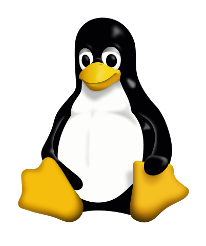
\includegraphics[scale=0.4]{./src/tux.png}
                \hspace*{5cm}
                \textit{Tux, la mascotte de linux}
            \end{figure}
        \end{frame}
        \subsection{Distro ?}
        \begin{frame}
            \frametitle{Distro ?}
            \only<1>{
                \begin{itemize}
                    \item Distro signifie \emph{distribution}
                \end{itemize}
                \begin{definition}
                    Une distribution est un ensemble cohérent de programmes, de services
                    et d'applications construits autour du noyau linux.
                \end{definition}
                \begin{itemize}
                    \item Plusieurs milliers de distribution
                    \item On peut créer la sienne !
                    \item Certaines sont gratuites, d'autres payantes
                    \item Certaines Open Source, d'autre non
                \end{itemize}
            }
            \only<2>{
                Voici une liste (non exhaustive) de distributions
                \begin{itemize}
                    \item Ubuntu (et ses variantes)
                    \item Debian
                    \item Archlinux
                    \item Pop!\_OS
                    \item Manjaro
                    \item Slackware
                    \item Gentoo
                    \item RedHatLinux (Fedora, CentOS...)
                \end{itemize}
                Notez que certaines distribution ne sont pas recommandées aux débutants 
            }
            \only<3>{
                Voici celles que je recommande :\\
                \textbf{Installation aisée}
                \begin{itemize}
                    \item Pop!\_OS
                    \item LinuxMint
                    \item OpenSuse
                \end{itemize}
                \textbf{Installation moyenne}
                \begin{itemize}
                    \item Debian
                    \item Fedora
                    \item CentOS/RockyLinux/AlmaLinux
                \end{itemize}
                \textbf{Installation complexe}
                \begin{itemize}
                    \item Archlinux
                    \item Gentoo
                    \item Slackware
                \end{itemize}
            }
        \end{frame}
        \subsection{Comment choisir un OS ?}
        \begin{frame}
            \frametitle{Comment choisir un OS ?}
            TODO : GRAPHE
        \end{frame}
    \section{Première installation}
        \begin{frame}
            \frametitle{Première installation}
            Linux peut être installé sur pleins de matériels différents :
            \begin{itemize}
                \item Ordinateur
                \item Calculatrice
                \item Robot
                \item etc.
            \end{itemize}
            Nous installerons Linux sur un micro-ordinateur, la "Raspberry Pi".
            Ce micro-ordinateur est utilisé dans pleins de domaines différents : industrie, domotique, micro-services...
        \end{frame}
        \begin{frame}
            \frametitle{Raspberry Pi ?}
            Voici à quoi ressemble une Raspberry Pi.
            \begin{figure}
                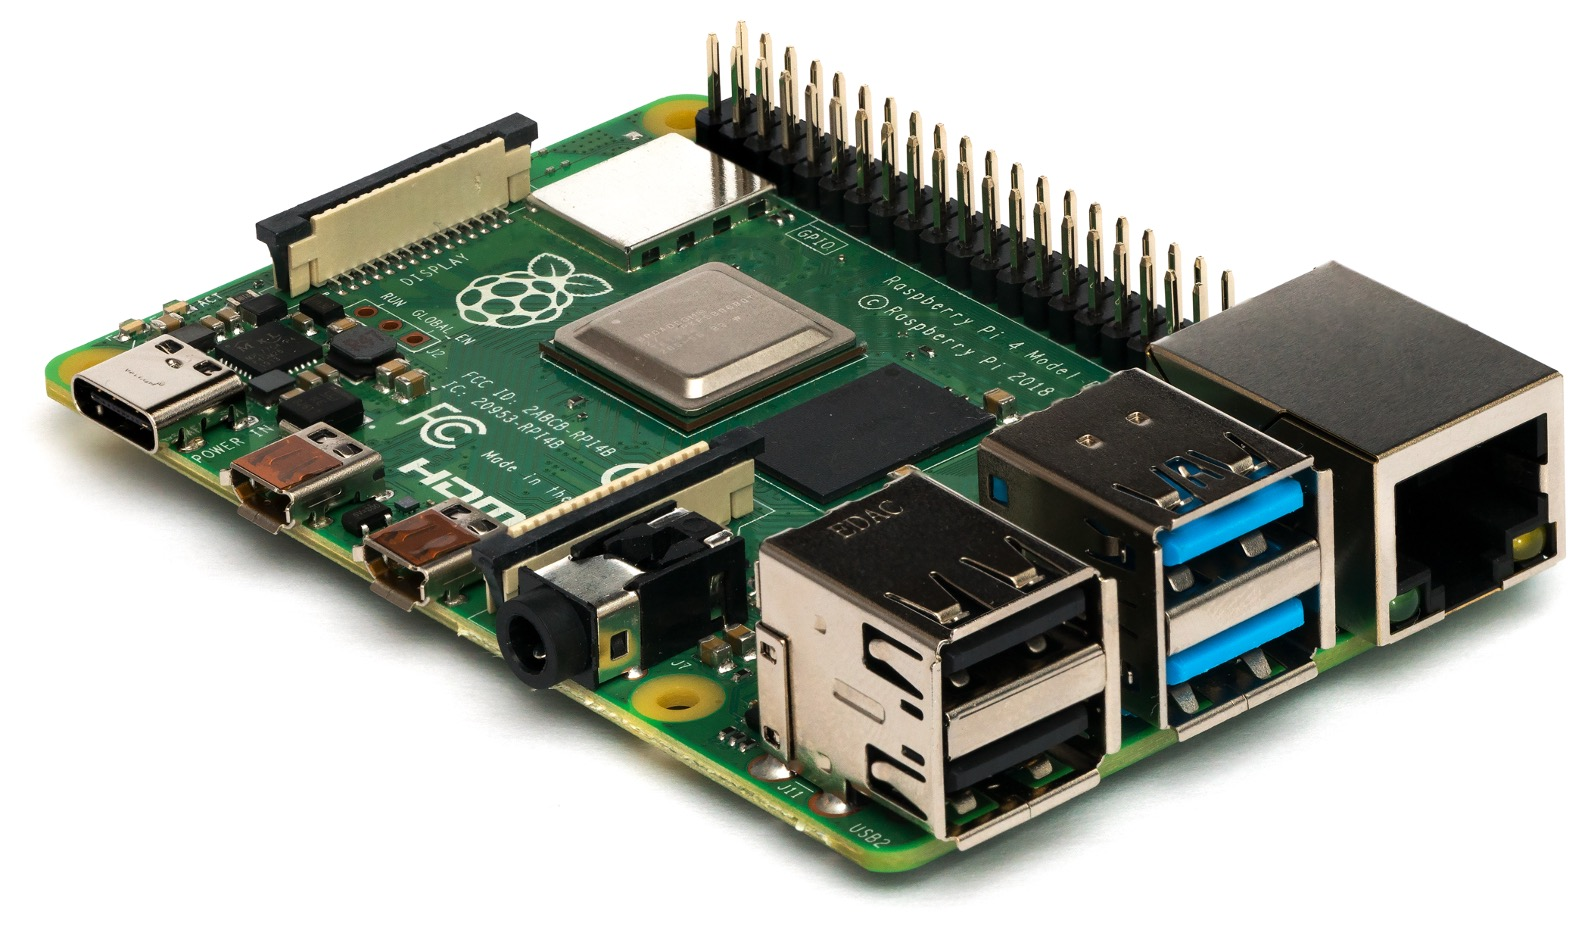
\includegraphics[scale=0.07]{./src/raspberrypi.jpg}
                \caption[]{Raspberry Pi}
            \end{figure}
            Celles que nous utiliserons seront protégées dans une boite en plastique rigide.
        \end{frame}
        \begin{frame}
            \frametitle{Boot Linux}
            Afin de \textbf{boot} une Raspberry Pi sur Linux, nous utiliserons une carte SD. Toutefois, il existe pleins de façons différentes de boot sur linux. On utilise souvent, pour la plupart des ordinateurs, une clef USB. Toutefois, on peut utiliser beaucoup de media (floppy disk, USB,...), ainsi que par le réseau.
        \end{frame}
    \section{Prise en main}
        \begin{frame}
            \frametitle{Prise en main}
        \end{frame}
    \section{Premières utilisations}
        \begin{frame}
                \frametitle{Premières utilisations}
        \end{frame}
    \section{Install, boot et config}
        \begin{frame}
            \frametitle{Install, boot et config}
        \end{frame}
\end{document}